\documentclass{beamer}
%
% Choose how your presentation looks.
%
% For more themes, color themes and font themes, see:
% http://deic.uab.es/~iblanes/beamer_gallery/index_by_theme.html
%
\mode<presentation>
{
  \usetheme{CambridgeUS}      % or try Darmstadt, Madrid, Warsaw, ...
  \usecolortheme{default} % or try albatross, beaver, crane, ...
  \usefonttheme{default}  % or try serif, structurebold, ...
  \setbeamertemplate{navigation symbols}{}
  \setbeamertemplate{caption}[numbered]
} 

\usepackage[english]{babel}
\usepackage[utf8x]{inputenc}
\usepackage{tikz}
\usetikzlibrary{trees}

% Set the overall layout of the tree
\tikzstyle{level 1}=[level distance=3cm, sibling distance=2.5cm]
\tikzstyle{level 2}=[level distance=3.5cm, sibling distance=1.2cm]
\tikzstyle{level 3}=[level distance=3cm, sibling distance=0.6cm]

% Define styles for bags and leafs
\tikzstyle{bag} = [text width=2em, text centered]
\tikzstyle{end} = [circle, minimum width=3pt,fill, inner sep=0pt]

\title{ENGG2430D Tutorial 6}
\author{Zhibo Yang}
\institute{\textit{Department of Information Engineering \\ The Chinese University of Hong Kong}}
\date{\textit{March 3, 2015}}

\begin{document}

\begin{frame}
\titlepage
\end{frame}

% automatically generated outline.
\begin{frame}{Outline}
  \tableofcontents
\end{frame}

\section{Homework 2}
\subsection{Problem 1}
\begin{frame}
\center \huge Homework 2
\end{frame}

\begin{frame}{Problem 1: Independence}
Assuming $A$, $B$, $C$ are \textbf{independent}, with $P(A)=0.1$, $P(B)=0.2$, $P(C)=0.3$, compute:\\
\vspace{0.3cm}
\begin{enumerate}[\hspace{0.5cm}1.]
        %\begin{enumerate}[1.]
    \item $P(A\cap B)$.\\
    \textbf{Solution:} $P(A)P(B)=0.02$
    \item $P(A\cup B)$. \\
    \textbf{Solution:} $P(A)+P(B)-P(A)P(B)=0.28$
    \item $P(A\cup B \cup C)$.\\
    \textbf{Solution:} $P(A)+P(B)+P(C)-P(A)P(B)-P(B)P(C)-P(A)P(C)+P(A)P(B)P(C)=0.496$
    \item $P((B\cup C)^c\cap A)$. \\
    \textbf{Solution:} $P(A)-P(A\cap B)-P(A\cap C)+P(A\cap B\cap C)=0.056$
        %\end{enumerate}
\end{enumerate}
\end{frame}

\subsection{Problem 2}
\begin{frame}{Problem 2: Bayes' Formula}
Solve the following questions.
\vspace{0.3cm}
    \begin{enumerate}[\hspace{0.5cm}1.]
    \item Suppose that $P(E)=0.3$, $P(F)=0.6$, and $P(E\cap F)=0.1$. Compute $P(E|F)$. \\
    \textbf{Solution:} $P(E|F)=P(E\cap F)/P(F)=1/6$
    \item Suppose that $P(E)=0.3$, $P(F)=0.6$, and that $E$ and $F$ are independent events. Compute $P(E|F)$.  \\
    \textbf{Solution:} $P(E|F)=P(E\cap F)/P(F)=(P(E)P(F))/P(F)=P(E)=0.3$
    \end{enumerate}
\end{frame}

\subsection{Problem 3}
\begin{frame}{Problem 3: Independence \& Bayes' Formula}
Assume $A$ and $B$ are independent events with $P(A)=0.1$ and $P(B)=0.4$. Let $C$ be the event that \textbf{at least one} of $A$ or $B$ occurs, and let $D$ be the event that \textbf{exactly one} of $A$ or $B$ occurs.
    \vspace{0.3cm}
    \begin{enumerate}[\hspace{0.5cm}1.]
        \item Find $P(C)$.\\
        \textbf{Solution:} The event $C$ is just the union of $A$ and $B$, so $P(C)=P(A\cup B)=P(A)+P(B)-P(A)P(B)=0.46$
        \item Find $P(D)$. \\
        \textbf{Solution:} We can see from the Venn diagram that $D$ consists of the union of $A$ and $B$ minus the overlap. Thus, $P(D)=P(A\cup B)-P(A\cap B)=0.42$
    \end{enumerate}
\end{frame}

\begin{frame}{Problem 3: Independence \& Bayes' Formula (cont'd)}
    \begin{enumerate}[\hspace{0.5cm}3.]
        \item Find $P(A|D)$ and $P(D|A)$.\\
        \textbf{Solution:} $P(A|D)=P(A\cap D)/P(D)=(P(A)-P(A\cap B))/P(D)=1/7$. $P(D|A)=P(A\cap D)/P(A)=0.6$
        \item Determine whether $A$ and $D$ are independent.\\
        \textbf{Solution:} Since $P(A|D)\neq P(A)$, $A$ and $D$ are not independent.
    \end{enumerate}
    \vspace{5cm}
\end{frame}

\subsection{Problem 4}
\begin{frame}{Problem 4: De Morgan's Law}
\begin{block}{}
Prove one of the De Morgan' laws: let $S_k$, $1\leq k\leq n$, be $n$ sets, then $\left(\cap_{k=1}^n S_k\right)^c = \cup_{k=1}^n S^c_k$.\\
\end{block}
\vspace{0.3cm}
\textbf{Solution:}\\\vspace{0.2cm}
If $x\in (\cap_{k=1}^nS_k)^c$, meaning $x\notin \cap_{k=1}^nS_k$, there exits $1\leq K\leq n$, such that $x\notin S_K$, i.e. $x\in S_K^c$. Then we can get $x\in \cup_{k=1}^nS_k^c$. $\Rightarrow (\cap_{k=1}^nS_k)^c \subseteq \cup_{k=1}^nS_k^c$.\\
\vspace{0.2cm}
If $x\in \cup_{k=1}^nS_k^c$, meaning there exists $1\geq K\leq n$, such that $x\notin S_K$, then we can get $x\notin \cap_{k=1}^nS_k$, i.e. $x\in (\cap_{k=1}^nS_k)^c$. $\Rightarrow  \cup_{k=1}^nS_k^c \subseteq (\cap_{k=1}^nS_k)^c$\\
\vspace{0.2cm}
Then we can obtain $(\cap_{k=1}^nS_k)^c = \cup_{k=1}^nS_k^c$
\end{frame}

\subsection{Problem 5}
\begin{frame}{Problem 5: Bayes' Formula}
    \begin{block}{}
    Finalphobia is a rare disease in which the victim has the delusion that he or she is being subjected to an intense mathematical examination. 
    \begin{itemize}
        \item A person selected uniformly at random has finalphobia with probability $1/200$.
        \item A person with finalphobia has shaky hands with probability $19/20$. 
        \item A person without finalphobia has shaky hands with probability $1/20$. 
    \end{itemize}
    What is the probablility that a randomly-selected person has finalphobia, given that he or she has shaky hands? \\
    \end{block}
    \vspace{0.3cm}
    \textbf{Solution:} Let $F$ be the event that the randomly-selected person has finalphobia, and let $S$ be the event that he or she has shaky hands. The probability that a person has finalphobia, given that he or she has shaky hands is: 
\end{frame}

\begin{frame}{Problem 5: Bayes' Formula(cont'd)}
    \begin{align}
        P(F|S)=&\frac{P(F\cap S)}{P(S)}\notag\\
        =&\frac{P(S|F)P(F)}{P(S)}\notag\\
        =&\frac{P(S|F)P(F)}{P(F^c)P(S|F^c)+P(F)P(S|F)}\notag\\
        =&\frac{\frac{19}{20}\frac{1}{200}}{\frac{199}{200}\frac{1}{20}+\frac{1}{200}\frac{19}{20}}\notag\\
        =&\frac{19}{218}\notag
    \end{align}
\end{frame}

\section{Homework 3}
\subsection{Problem 1}
\begin{frame}
\center \huge Homework 3
\end{frame}

\begin{frame}{Problem 1}
Please show that two events, A and B, are not independent if their rela- tionship is characterized by either one of the diagrams in Fig. \ref{fig1}.
\begin{figure}
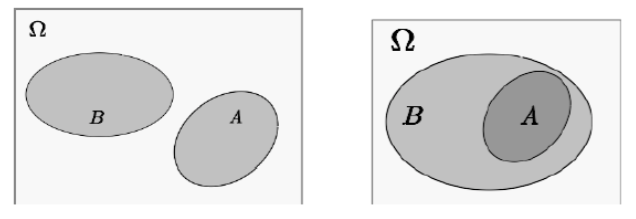
\includegraphics[width=10cm]{fig1}
\caption{\label{fig1}two relationships between A and B}
\end{figure}
\end{frame}

\begin{frame}{Problem 1 (cont'd)}
\textbf{Solution:}
When the relationship is characterized by the diagram on the left, $A$ and $B$ are disjoint, so $P(AB) = 0$, but $P(A)$ and $P(B)$ are positive, then $P(A)P(B)\neq P(AB)$.
\vspace{0.2cm}
When the relationship is characterized by the diagram on the right, $A\subset B$, meaning $A\cap B = A$, so $P(AB) = P(A)$, with the fact that $P(B) < 1$, then $P(AB) < P(A)P(B)$.
\vspace{0.2cm}
We can have that $A$ and $B$ are not independent for both cases.
\vspace{4cm}
\end{frame}

\subsection{Problem 2}
\begin{frame}{Problem 2}
\begin{block}{}
Given a random variable $X$, whose distribution is given by
$$P(X=k)= \frac{\lambda^ke^{-\lambda}}{k!}, \quad k = 0,1,2,...$$
where $\lambda$ is a specified constant. Suppose we know that $\lambda = E(X) = Var(X)$. Now we define a new random variable $Y = X^2$, please compute the expectation of Y, i.e., $E[Y]$.\\
\end{block}
\textbf{Solution.} For any random variable $X$, we can have $$Var[X] = E[X^2]-(E[X])^2.$$
Then $E[Y] = E[X^2] = Var[X]+(E[X])^2 = \lambda +\lambda^2.$\\
\vspace{0.2cm}
\textbf{P.S: }$X$ is actually the Poisson random variable.
\end{frame}

\subsection{Problem 3}
\begin{frame}{Problem 3}
Consider a coin. When you flip it, it will show a head with probability $p=\frac{1}{3}$ and a tail
     with probability $q=1-p=\frac{2}{3}$. Suppose the results of different flips are independent.
        Calculate the PMF, expectation and variance of the random variable $X$ in the following cases.
        \begin{enumerate}[(a)]
            \item (Bernoulli) $X$ is the number of heads when you flip the coin once. \\
            {\bf Solution:} The PMF function is
            \begin{equation}
            \nonumber
            p_{X}(x) = \left\{
                         \begin{array}{ll}
                           p=\frac{1}{3}, & \hbox{$X=1$;} \\
                           q=\frac{2}{3}, & \hbox{$X=0$.}
                         \end{array}
                       \right.
            \end{equation}
            The expectation is \[E[X] = p = \frac{1}{3}.\]
            The variance is \[\text{var}(X) = pq = \frac{2}{9}.\]
        \end{enumerate}
\end{frame}
\begin{frame}{Problem 3 (cont'd)}
    \begin{enumerate}[(b)]
        \item (Binomial)  $X$ is the number of heads when you flip the coin 4 times. \\

        {\bf Solution:} The PMF function is \[p_X(x)=\binom{4}{x}p^xq^{4-x} = \binom{4}{x}\left(\frac{1}{3}\right)^x
         \left(\frac{2}{3}\right)^{4-x}, x=0,1,2,3,4.\] More specifically,
        the PMF is shown in the following table.
        \begin{center}
        \begin{tabular}{|c|c|c|c|c|c|}
          \hline
          % after \\: \hline or \cline{col1-col2} \cline{col3-col4} ...
          $x$ & 0 & 1 & 2 & 3 & 4 \\
          \hline
          $p_{X}(x)$ & $\frac{16}{81}$ & $\frac{32}{81}$ & $\frac{24}{81}$ & $\frac{8}{81}$ & $\frac{1}{81}$ \\
          \hline
        \end{tabular}
        \end{center}

        The expectation is \[E[X] = 4p = \frac{4}{3}.\]
        The variance is \[\text{var}(X)=4pq = \frac{8}{9}.\]
    \end{enumerate}
\end{frame}
\begin{frame}{Problem 3 (cont'd)}
    \begin{enumerate}[(c)]
        \item (Geometric) $X$ is the number of flips until you see a head the first time. \\
             {\bf Solution:} The PMF function is \[p_X(x)=q^{x-1}p = \frac{2^{x-1}}{3^x}, x=1,2,3, \cdots\]
            The expectation is \[E[X] = \frac{1}{p} = 3.\]
            The variance is \[\text{var}(X)= \frac{q}{p^2} = 6.\]
    \end{enumerate}
\end{frame}

\subsection{Problem 4}
\begin{frame}{Problem 4}
let us consider throwing a fair die twice. Throwing the die once will equally likely show all 6 results (1, 2, 3, 4, 5, or 6 dots).
         Suppose the results of the first throw and the second throw are independent. And define the
         following random variables.
         \begin{eqnarray}
         && X_1 = \{\text{The number of dots in the first throw}\} \nonumber \\
         && X_2 = \{\text{The number of dots in the second throw}\} \nonumber \\
         && Z = X_1 - X_2 \nonumber
         \end{eqnarray}
        \vspace{-0.5cm}
        \begin{enumerate}[(a)]
            \item Find the PMF of $X_1$, $X_2$, and $Z$, i.e., $p_{X_1}(x_1)$, $p_{X_2}(x_2)$ and $p_{Z}(z)$. \\
            {\bf Solution:} The PMF function is
            \[p_{X_1}(x_1) = \frac{1}{6}, x_1 = 1,2,3,4,5,6.\]
            \[p_{X_2}(x_2) = \frac{1}{6}, x_2 = 1,2,3,4,5,6.\]
        \end{enumerate}
\end{frame}
\begin{frame}{Problem 4 (cont'd)}
\begin{center}
\begin{tabular}{|c|c|c|c|c|c|c|c|c|c|c|c|}
  \hline
  % after \\: \hline or \cline{col1-col2} \cline{col3-col4} ...
  $z$ & $-5$ & $-4$ & $-3$ & $-2$ & $-1$ & 0 & 1 & 2 & 3 & 4 & 5 \\
  \hline
  $p_{Z}(z)$ & $\frac{1}{36}$ & $\frac{2}{36}$ & $\frac{3}{36}$ & $\frac{4}{36}$ & $\frac{5}{36}$
  & $\frac{6}{36}$ & $\frac{5}{36}$ & $\frac{4}{36}$ & $\frac{3}{36}$ & $\frac{2}{36}$ & $\frac{1}{36}$\\
  \hline
\end{tabular}
\end{center}
    \begin{enumerate}[(b)]
        \item Find the expectation and variance of $X_1$, $X_2$ and $Z$. \\
            {\bf Solution:}
            \[E[X_1]=E[X_2]=\frac{7}{2}, E[Z]=0.\]
            \[\text{Var}(X_1)=\text{Var}(X_2)= \frac{35}{12}, \text{Var}(Z)= \frac{35}{6}.\]
    \end{enumerate}
\end{frame}
\begin{frame}{Problem 4 (cont'd)}
    \begin{enumerate}[(a)]
    \setcounter{enumi}{2}
        \item Find the joint PMF of $X_1$ and $Z$, i.e., $p_{X_1,Z}(x_1,z)$. \\
        \begin{center}
            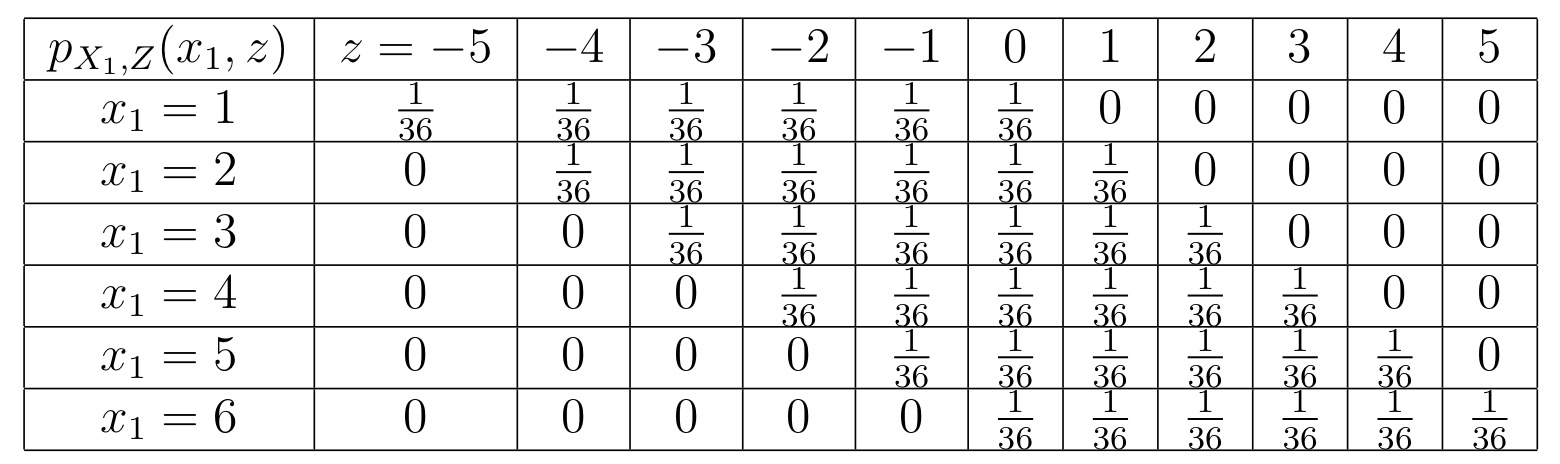
\includegraphics[width=9cm]{fig2}
        \end{center}
        \item Determine whether $X_1$ and $Z$ are independent or not. \\
        {\bf Solution:} Consider $X_1=1, Z=1$. Since \[p_{X_1}(1)=\frac{1}{6}, p_{Z}(1)=\frac{5}{36},
         p_{X_1,Z}(1,1)=0,\] we get that \[p_{X_1,Z}(1,1) \neq p_{X_1}(1)p_{Z}(1).\]
         Therefore, $X_1$ and $Z$ are not independent.
    \end{enumerate}
\end{frame}

\subsection{Problem 5}
\begin{frame}{Problem 5}
Given two \textbf{independent} random variables $X_1$ and $X_2$, we know that they follow the geometric distribution with parameters $p_1$ and $p_2$ respectively. Now we define another random variable $$X = \min\{X_1,X_2\}.$$
\vspace{-0.5cm}
        \begin{enumerate}[(a)]
            \item Given a positive integer $k$, please compute the probabilities that $X_1$ and $X_2$ are no larger than $k$ respectively, i.e.,
    $P(X_1 \leq k)$ and $P(X_2\leq k)$.\\
    {\bf Solution: }We know that $P(X_i = n) = (1-p_i)^{n-1}p_i$. Then
    $$P(X_i\leq k) = \sum_{n = 1}^kP(X_i = n) = \sum_{n = 1}^k(1-p_i)^{n-1}p_i = 1-(1-p_i)^k$$

we can have $P(X_1 \leq k) = 1-(1-p_1)^k$ and $P(X_2 \leq k) = 1-(1-p_2)^k$.
        \end{enumerate}
\end{frame}
\begin{frame}{Problem 5 (cont'd)}
    \begin{enumerate}[(b)]
        \item Please find the probability that $X$ is no larger than $k$, i.e., $P(X\leq k)$. Hint: $P(X_i\leq k)+ P(X_i> k) = 1$, $P(X> k) = P(X_1> k, {and } X_2> k)$ and use the fact that $X_1$ and $X_2$ are independent.\\
            {\bf Solution:}
            By the result in (a), we can have $P(X_i>k) = 1-P(X_i\leq k) = (1-p_i)^k.$ The next computation is as follows,
            \begin{align*}
            P(X> k) &= P(X_1> k, {and } X_2> k) \quad \text{By the definition of $X$.}\\
            &=P(X_1>k)P(X_2>k) \quad \text{By the independence of $X_1$ and $X_2$.}\\
            & =(1-p_1)^k(1-p_2)^k\\
            & = \left[(1-p_1)(1-p_2)\right]^k.
            \end{align*}
            And $$P(X\leq k) = 1-P(X>k) = 1-\left[(1-p_1)(1-p_2)\right]^k.$$
    \end{enumerate}
\end{frame}
\begin{frame}{Problem 5 (cont'd)}
    \begin{enumerate}[(c)]
        \item Next, compute $P(X = k)$. Hopefully you will find that $X$ is a geometric random variable.
        \begin{align*}
        P(X=k) &= P(X\leq k)- P(X\leq k-1)\\
        & = \left[(1-p_1)(1-p_2)\right]^{k-1}-\left[(1-p_1)(1-p_2)\right]^k\\
        & = \left[(1-p_1)(1-p_2)\right]^{k-1}\left[1-(1-p_1)(1-p_2)\right]
        \end{align*}
        By letting $ p = 1-(1-p_1)(1-p_2)$, we can have $P(X=k) = (1-p)^{k-1}p$. It is easy to see that $X$ is a geometric random variable with parameter $p$.
    \end{enumerate}
\end{frame}
\end{document}
